\documentclass[aps,pra,preprint,superscriptaddress,nofootinbib]{revtex4-2}

\usepackage[T1]{fontenc}
\usepackage{lmodern}
\usepackage{amsmath,amssymb}
\usepackage{booktabs}
\usepackage{graphicx}
\usepackage{hyperref}
\usepackage{microtype}

\graphicspath{{figures/}}
\hypersetup{
  colorlinks=true,
  linkcolor=blue,
  citecolor=blue,
  urlcolor=blue
}

\begin{document}

\title{Comprehensive Reproduction Report for the Nonsymmorphic Discrete Time Crystal Model}
\author{Reproduction notes, numerical implementation, and finite-size checks}
\affiliation{Local CUDA and H100 reproduction workflow}
\date{\today}

\begin{abstract}
This report summarizes the reproduction of the nonsymmorphic discrete time crystal model of Hu, Fu, Li, and Shen, Phys. Rev. Research 5, L032024 (2023). The work includes a reading-stage review of the mechanism, a noninteracting two-level reproduction with fourth-order Magnus and Runge--Kutta checks, and an interacting exact state-vector spin-chain reproduction with local and H100-ready workflows. The noninteracting reproduction confirms the special refined point \(\alpha_{13}=80.04624211689759\), where one-period return to the initial instantaneous eigenstate is suppressed and a robust two-period response appears. For the interacting chain, the final convention keeps the paper-label interaction strength \(J/\hbar\omega=0.2\) but applies a Pauli-operator scale factor of \(1/2\), so \(J_{\rm eff}=0.1\) in the implemented \(\sigma_x^i\sigma_x^{i+1}\) term. Under this convention the refined \(\alpha_{13}\) data show the expected lifetime enhancement from \(L=8\) to \(L=10\). The remaining unresolved discrepancy is that the detuned \(\alpha=81.60\) raw \(Z(n)\) trace decays much faster than the paper's Fig. 4(c) under both open and periodic boundary conditions, indicating that the paper's lifetime extraction, interaction normalization, or numerical protocol may differ from the current raw-observable implementation.
\end{abstract}

\maketitle

\section{Scope and Deliverables}

The target paper proposes a solvable route to discrete time-crystal (DTC) dynamics enforced by a nonsymmorphic dynamical symmetry. The reproduction was organized into four stages:
\begin{enumerate}
\item read and summarize the main paper and supplemental material;
\item reproduce the noninteracting two-level dynamics and compare fourth-order Magnus evolution with a Runge--Kutta benchmark;
\item reproduce the interacting spin-chain response with CUDA/PyTorch exact state-vector dynamics and HPC-ready parameter files;
\item collect the theory, numerical methods, figures, diagnostics, and open issues into the present comprehensive report.
\end{enumerate}

The main project artifacts are the reading report, the noninteracting reproduction report, the interacting reproduction report, the Python scripts, parameter JSON files, selected data tables, and the final report in this directory. The numerical code follows a simple function-based structure so that the physical assumptions are visible at the point of use.

\section{Model and DTC Mechanism}

The single-spin Hamiltonian used throughout the reproduction is
\begin{equation}
H_0(t)=\frac{1}{2}\Omega\sin(\omega t)\sigma_x+
\Omega\sin^2\left(\frac{\omega t}{2}\right)\sigma_y,
\label{eq:h0}
\end{equation}
with the dimensionless convention
\begin{equation}
\hbar=1,\qquad \omega=1,\qquad T=2\pi,\qquad
\Omega=\alpha/8.
\end{equation}
The paper's special parameters \(\alpha_n\) are selected by the nonsymmorphic dynamical symmetry. At these points the instantaneous eigenstates swap after one driving period and return only after two periods, producing a subharmonic response at half the drive frequency.

In the interacting stage the implemented chain Hamiltonian is
\begin{equation}
H(t)=\sum_{i=1}^{L}H_{0,i}(t)
+J_{\rm eff}\sum_{\langle i,j\rangle}\sigma_x^i\sigma_x^j.
\label{eq:hint}
\end{equation}
The final production convention is
\begin{equation}
J_{\rm paper}/\hbar\omega=0.2,\qquad
J_{\rm eff}=0.5J_{\rm paper}=0.1.
\label{eq:jconv}
\end{equation}
This distinction is important because the code multiplies explicit Pauli matrices, whereas the paper's wording uses spin operators. Directly using \(J=0.2\) as the Pauli-product coefficient was found to overdrive the many-body chain and to produce an unphysical early decay for \(L=10\) at refined \(\alpha_{13}\).

The initial state for the interacting runs is
\begin{equation}
|\psi(0)\rangle=\bigotimes_{i=1}^{L}|+x\rangle_i,
\end{equation}
matching the main text statement that the spins are initially polarized in the \(x\) direction. The monitored observables are
\begin{equation}
m_x(t)=\frac{1}{L}\sum_i
\langle \psi(t)|\sigma_x^i|\psi(t)\rangle
\end{equation}
and the stroboscopic signal
\begin{equation}
Z(n)=(-1)^n m_x(nT).
\end{equation}
The supplemental material also allows more general \(x\)-product states
\(\otimes_i |s_i,x\rangle\), but for global \(m_x\) such states can change the amplitude by partial cancellation. The all-\(+x\) state therefore gives the cleanest direct comparison with Fig. 4.

\section{Noninteracting Reproduction}

\subsection{Numerical method}

The noninteracting solver uses two independent time-evolution checks. The first is a fourth-order Gauss--Legendre Magnus integrator, chosen because it preserves the unitary structure more faithfully than a generic explicit integrator. The second is a classical fourth-order Runge--Kutta solver used as an independent benchmark. Both solvers evolve the same two-level Hamiltonian in Eq.~(\ref{eq:h0}).

The refined special point used in all later runs is
\begin{equation}
\alpha_{13}=80.04624211689759,
\end{equation}
which is close to the paper's tabulated value \(80.07\). The computed one-period return probability at this refined point is \(3.57\times10^{-18}\), consistent with nearly perfect swapping rather than one-period return.

\subsection{Results}

Figure~\ref{fig:nonint-sigmax} compares \(\langle\sigma_x(t)\rangle\) for the refined \(\alpha_{13}\) and detuned \(\alpha=81.60\). The refined parameter produces a clean half-frequency response over the plotted time window. The detuned parameter still has visible subharmonic character over short times, but the detailed waveform and spectrum shift away from the exact-\(\alpha_n\) behavior.

\begin{figure}
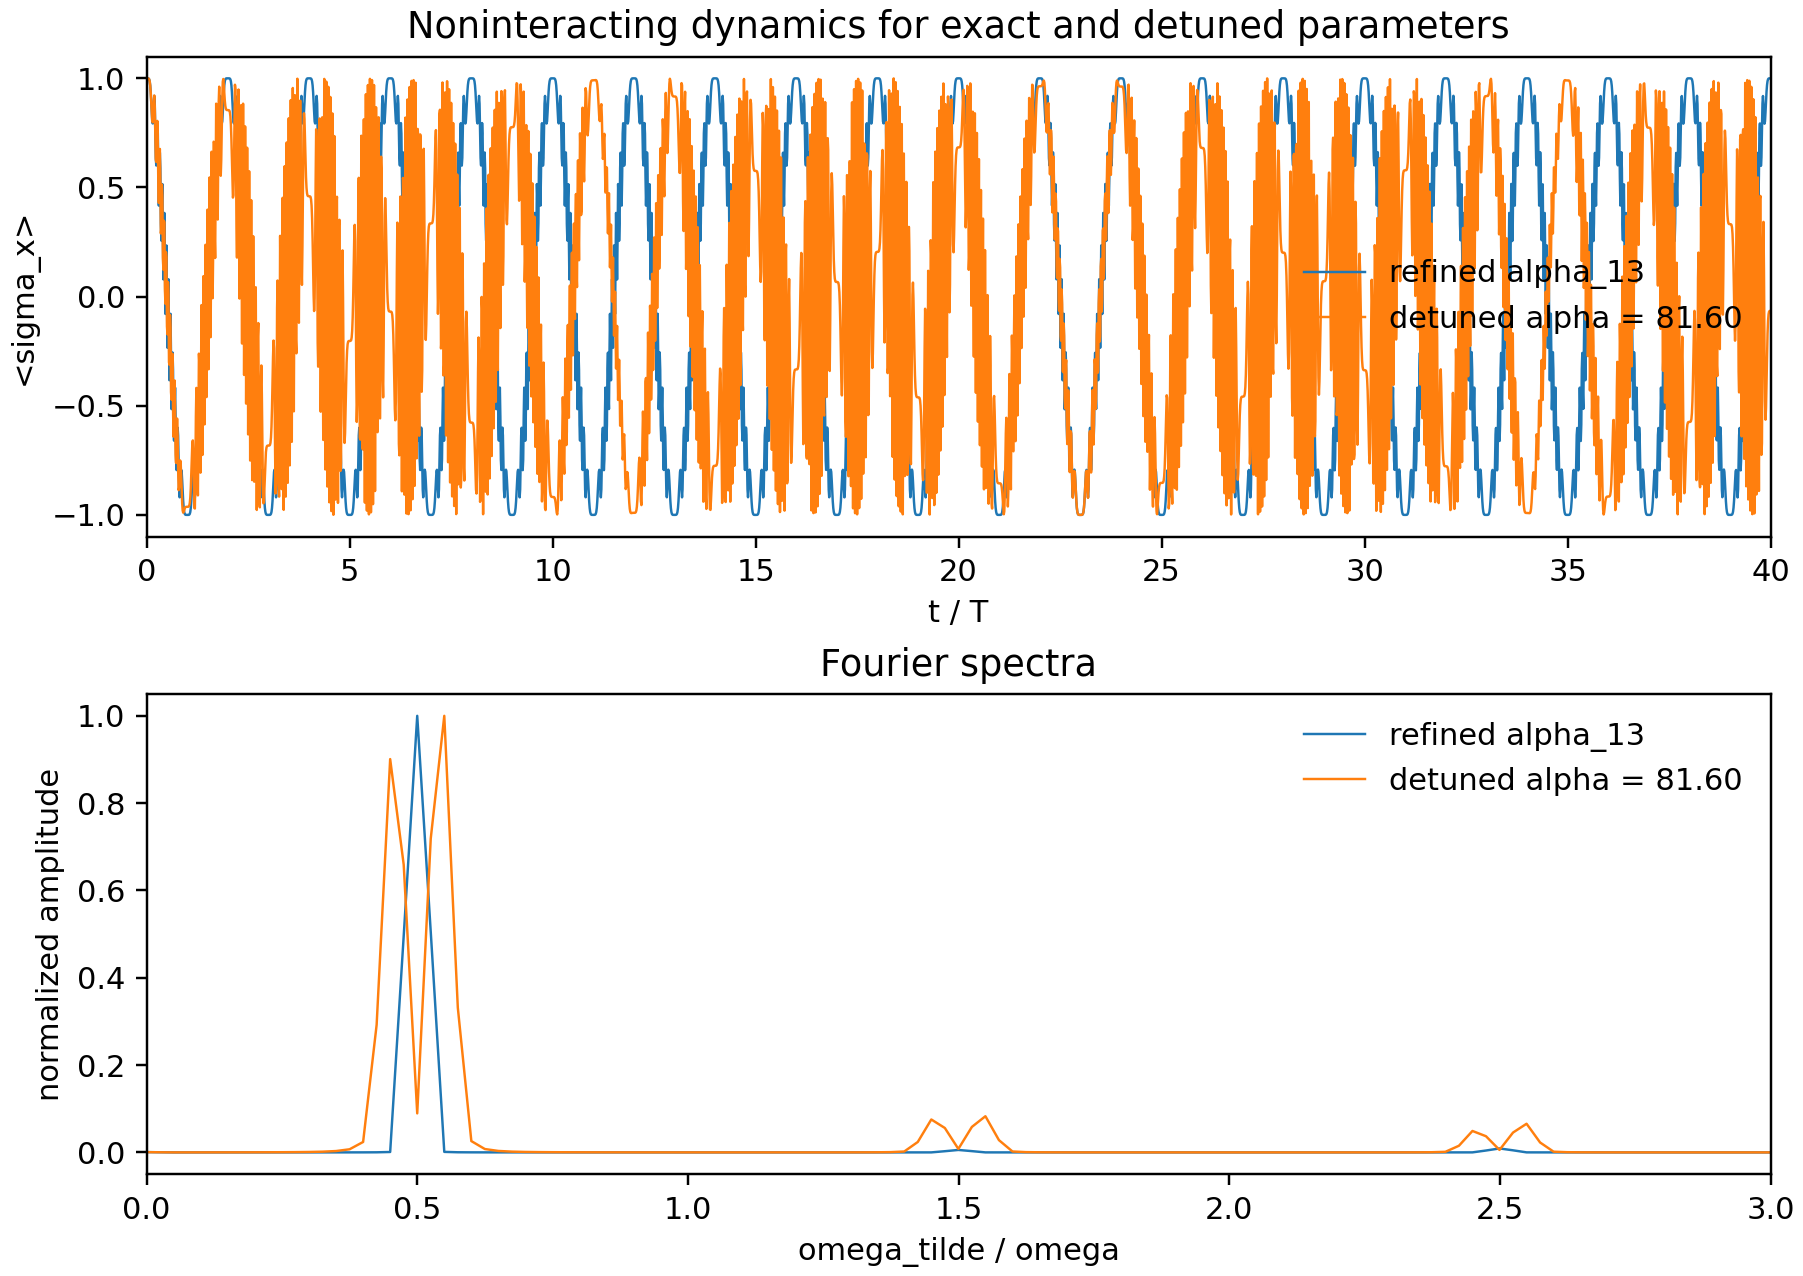
\includegraphics[width=0.92\linewidth]{noninteracting_sigma_x_parameter_comparison.png}
\caption{Noninteracting \(\sigma_x(t)\) comparison for refined \(\alpha_{13}\) and detuned \(\alpha=81.60\).}
\label{fig:nonint-sigmax}
\end{figure}

The fractional-period projection data in Fig.~\ref{fig:nonint-proj} sample \(0,T/4,T/2,3T/4\) within each period. This was added because stroboscopic-only plots can hide the intra-period exchange of instantaneous eigenstate weight.

\begin{figure}
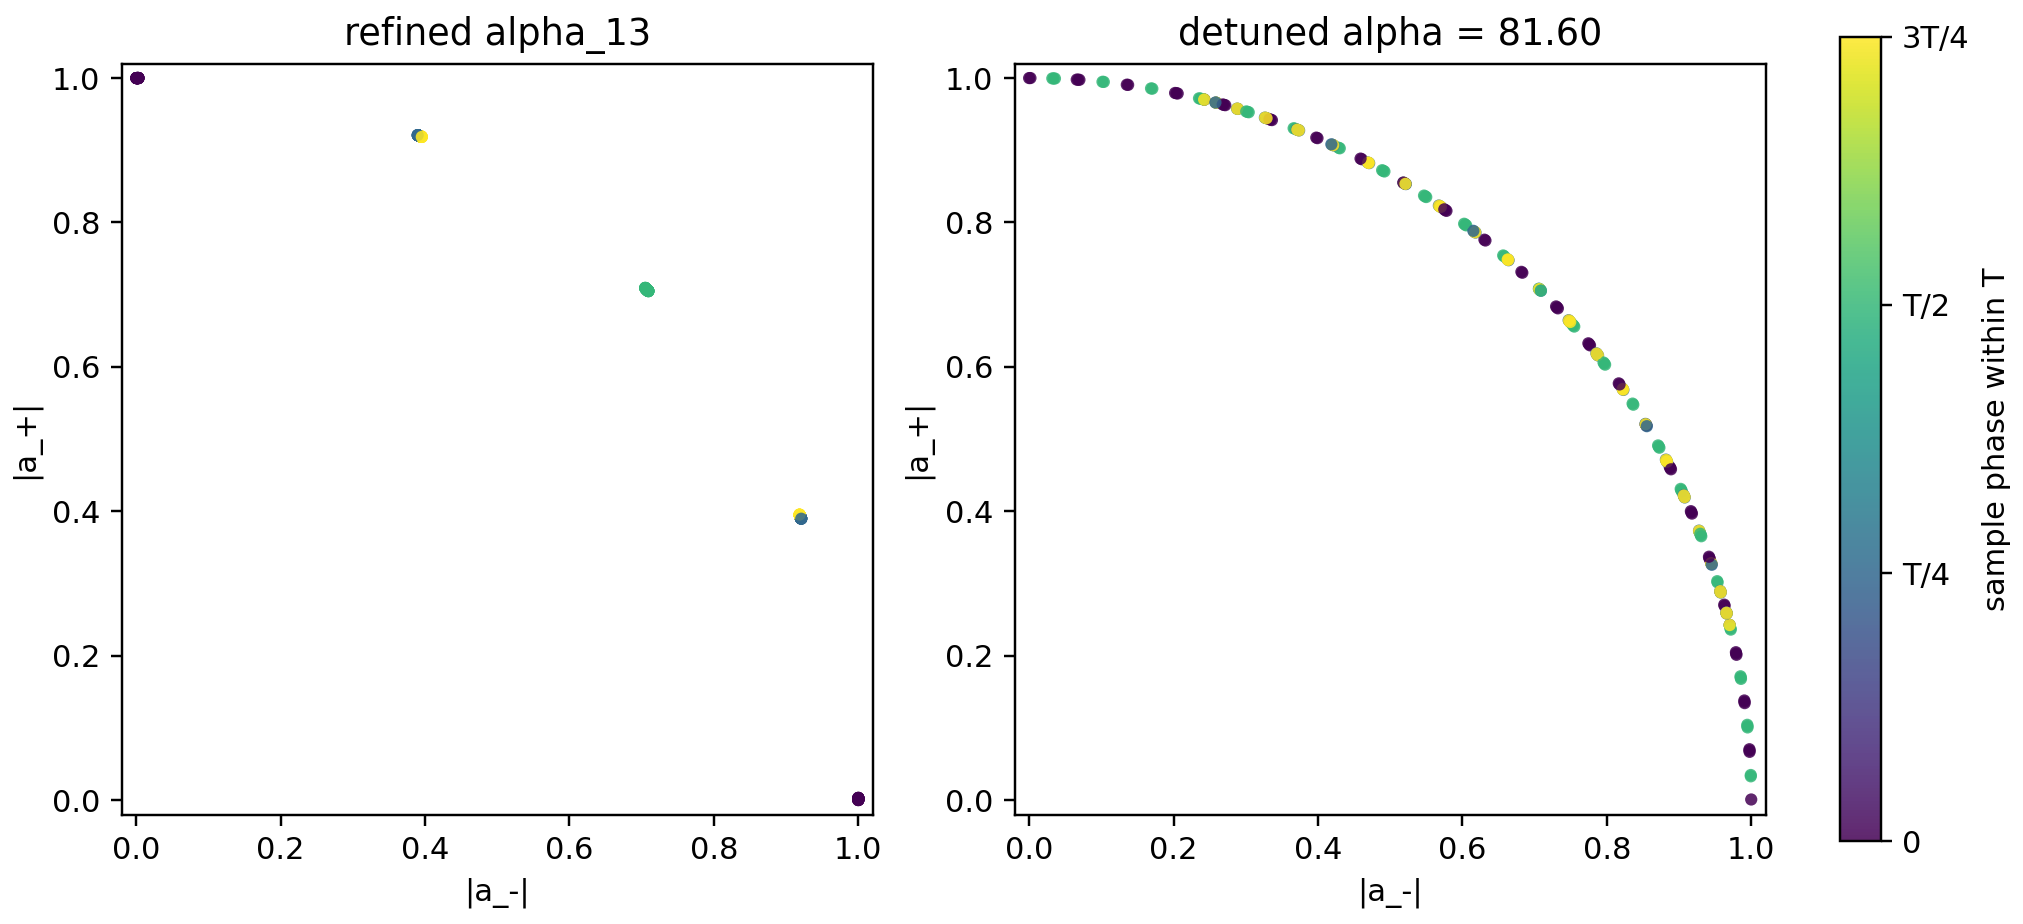
\includegraphics[width=0.92\linewidth]{noninteracting_fractional_projections_parameter_comparison.png}
\caption{Fractional-period projection comparison. Sampling within each period exposes the eigenstate exchange that is hidden in integer-period-only plots.}
\label{fig:nonint-proj}
\end{figure}

\begin{table}
\caption{Noninteracting solver diagnostics. Frequencies are normalized by the drive angular frequency.}
\label{tab:nonint-diagnostics}
\begin{ruledtabular}
\begin{tabular}{lcccc}
case & \(\alpha\) & Magnus norm drift & RK4 norm drift & dominant frequency \\
\hline
refined \(\alpha_{13}\) & 80.0462421169 & \(4.02\times10^{-5}\) & \(1.59\times10^{-3}\) & 0.49984 \\
detuned & 81.60 & \(3.92\times10^{-5}\) & \(1.79\times10^{-3}\) & 0.54983 \\
\end{tabular}
\end{ruledtabular}
\end{table}

The refined point also shows the expected two-period stroboscopic structure, as summarized in Fig.~\ref{fig:nonint-strobe}.

\begin{figure}
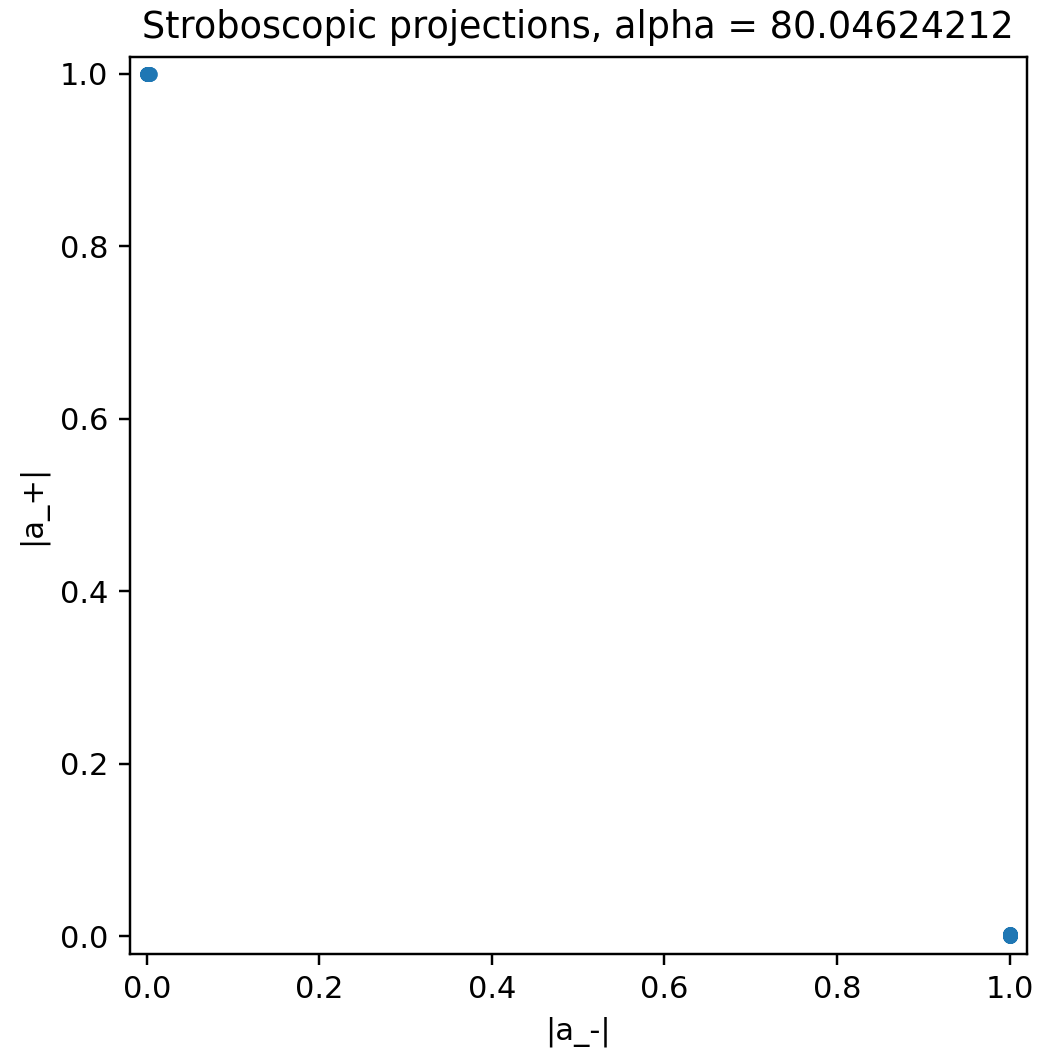
\includegraphics[width=0.86\linewidth]{noninteracting_stroboscopic_alpha_13.png}
\caption{Stroboscopic projection at refined \(\alpha_{13}\). The two-period structure follows from the nonsymmorphic dynamical symmetry.}
\label{fig:nonint-strobe}
\end{figure}

\section{Interacting Reproduction}

\subsection{Implementation and boundary conditions}

The interacting code evolves an exact state vector of dimension \(2^L\). The Hamiltonian action is implemented with bit-flip tensor indexing rather than building dense \(2^L\times2^L\) matrices for ordinary time traces. Long-time stroboscopic sampling uses a dense one-period Floquet operator and logarithmic sampling in \(n\), which makes \(10^{10}\)--\(10^{12}\) period checks feasible for \(L=8\) and \(L=10\).

Open boundary conditions use \(L-1\) nearest-neighbor bonds. Periodic boundary conditions add the final \(L,1\) bond and are controlled by the JSON parameter \texttt{boundary}. Periodic outputs carry a suffix so that they do not overwrite open-boundary results.

The H100 package and local code use the same parameter structure. The current main settings are \(L=10\), open boundary conditions, \(\alpha=81.60\) and refined \(\alpha_{13}\), \(J_{\rm paper}=0.2\), \(\texttt{interaction\_operator\_scale}=0.5\), and \(120\) steps per driving period for the one-period Floquet construction.

\subsection{Short-time response}

The first interacting check reproduces the half-drive-frequency response of \(m_x(t)\) over the first 40 periods. Figure~\ref{fig:int-trace} shows the \(L=10\) time traces. The corresponding spectra have dominant normalized frequency \(0.4998\) for both the refined and detuned parameters over this short window.

\begin{figure}
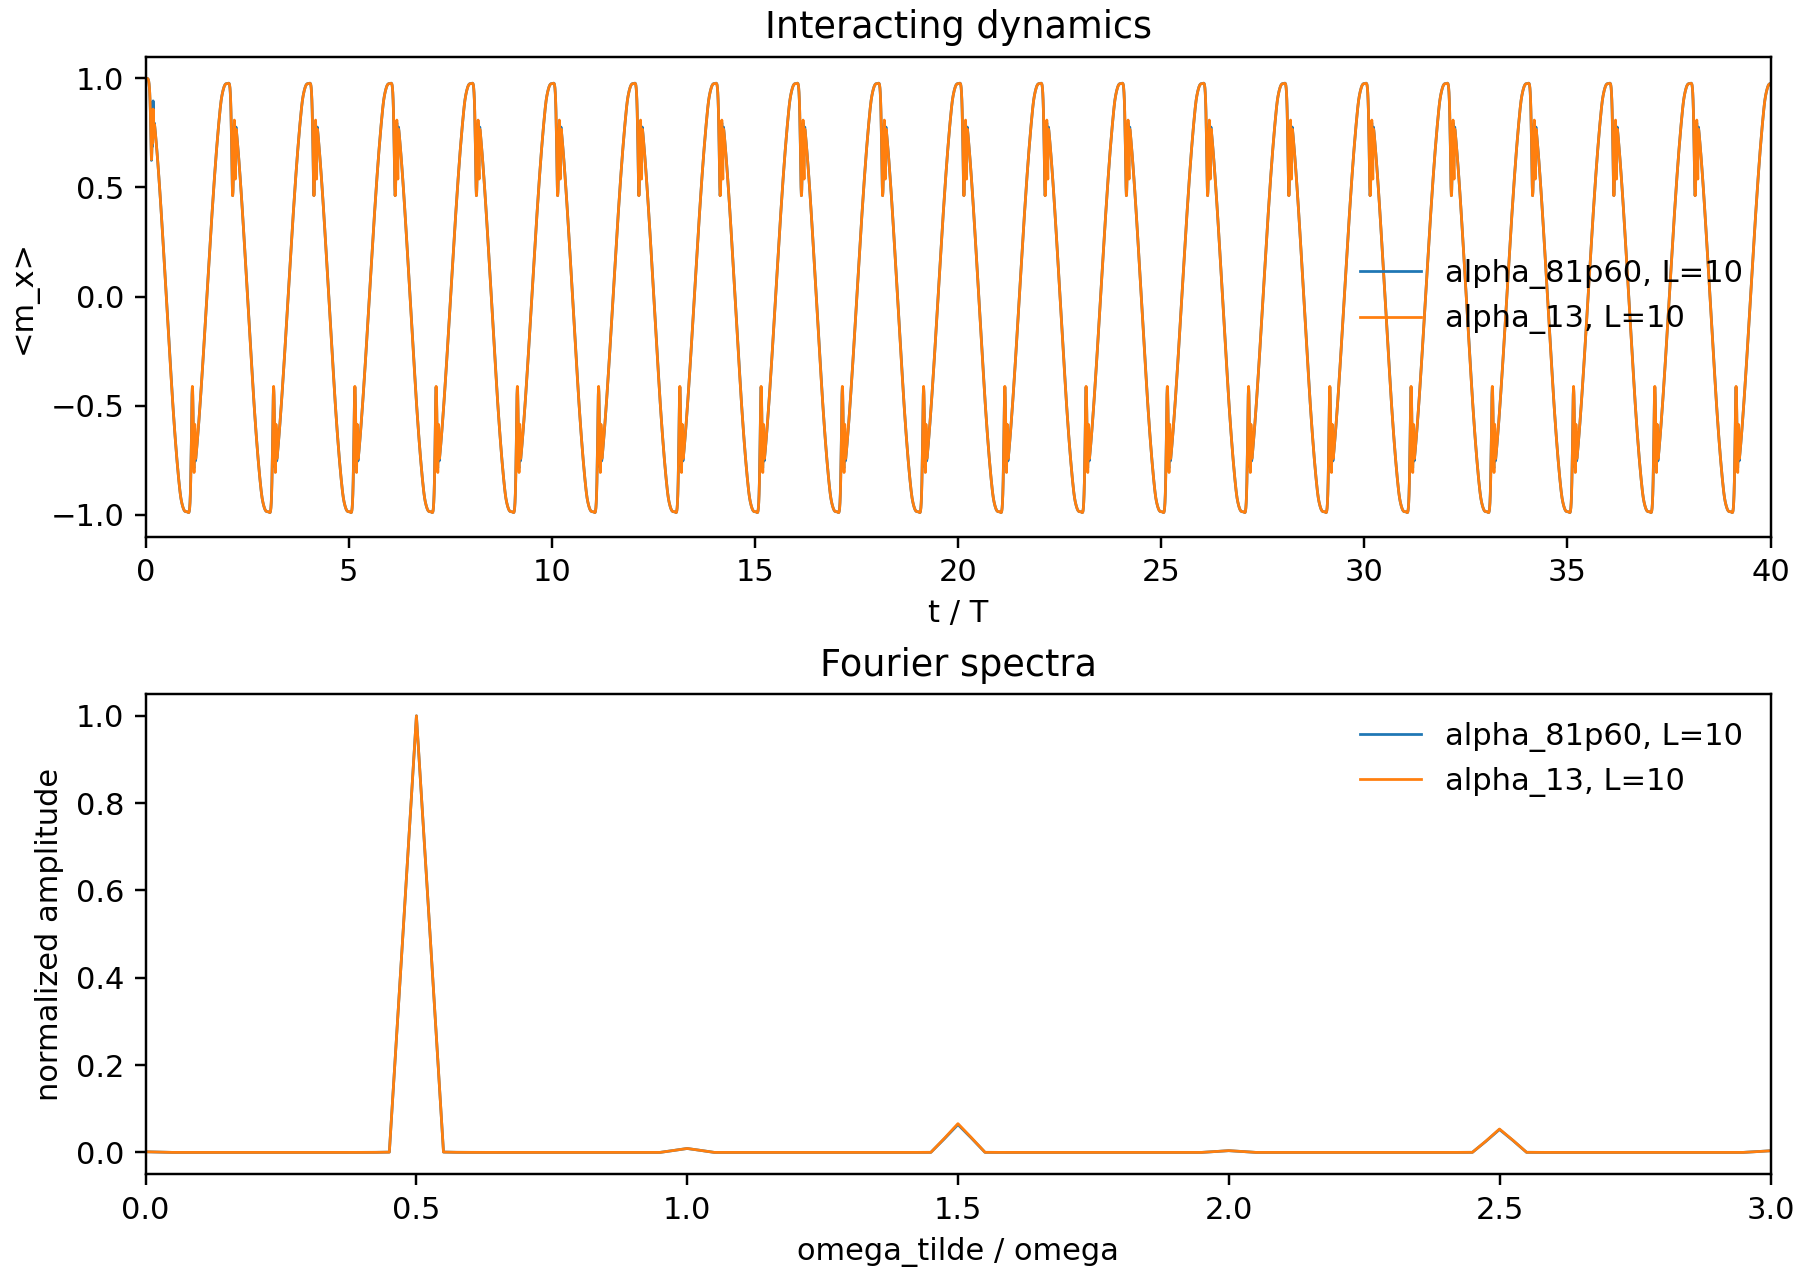
\includegraphics[width=0.92\linewidth]{interacting_mx_trace_comparison_l10.png}
\caption{Interacting \(L=10\) short-time \(m_x(t)\) traces. Short-time period doubling is visible for both refined \(\alpha_{13}\) and detuned \(\alpha=81.60\).}
\label{fig:int-trace}
\end{figure}

\subsection{Interaction convention check}

The most important debugging step was the comparison in Fig.~\ref{fig:jconv}. If the paper-label \(J=0.2\) is used directly as a Pauli-product coefficient, the \(L=10\), refined-\(\alpha_{13}\) signal falls below \(Z=0.8\) by \(n=160\). This contradicts the expected stability and the paper-scale result. With the spin-operator convention \(J_{\rm eff}=0.1\), the same \(L=10\) run stays above \(Z=0.9\) through the sampled \(10^{10}\) periods.

\begin{figure}
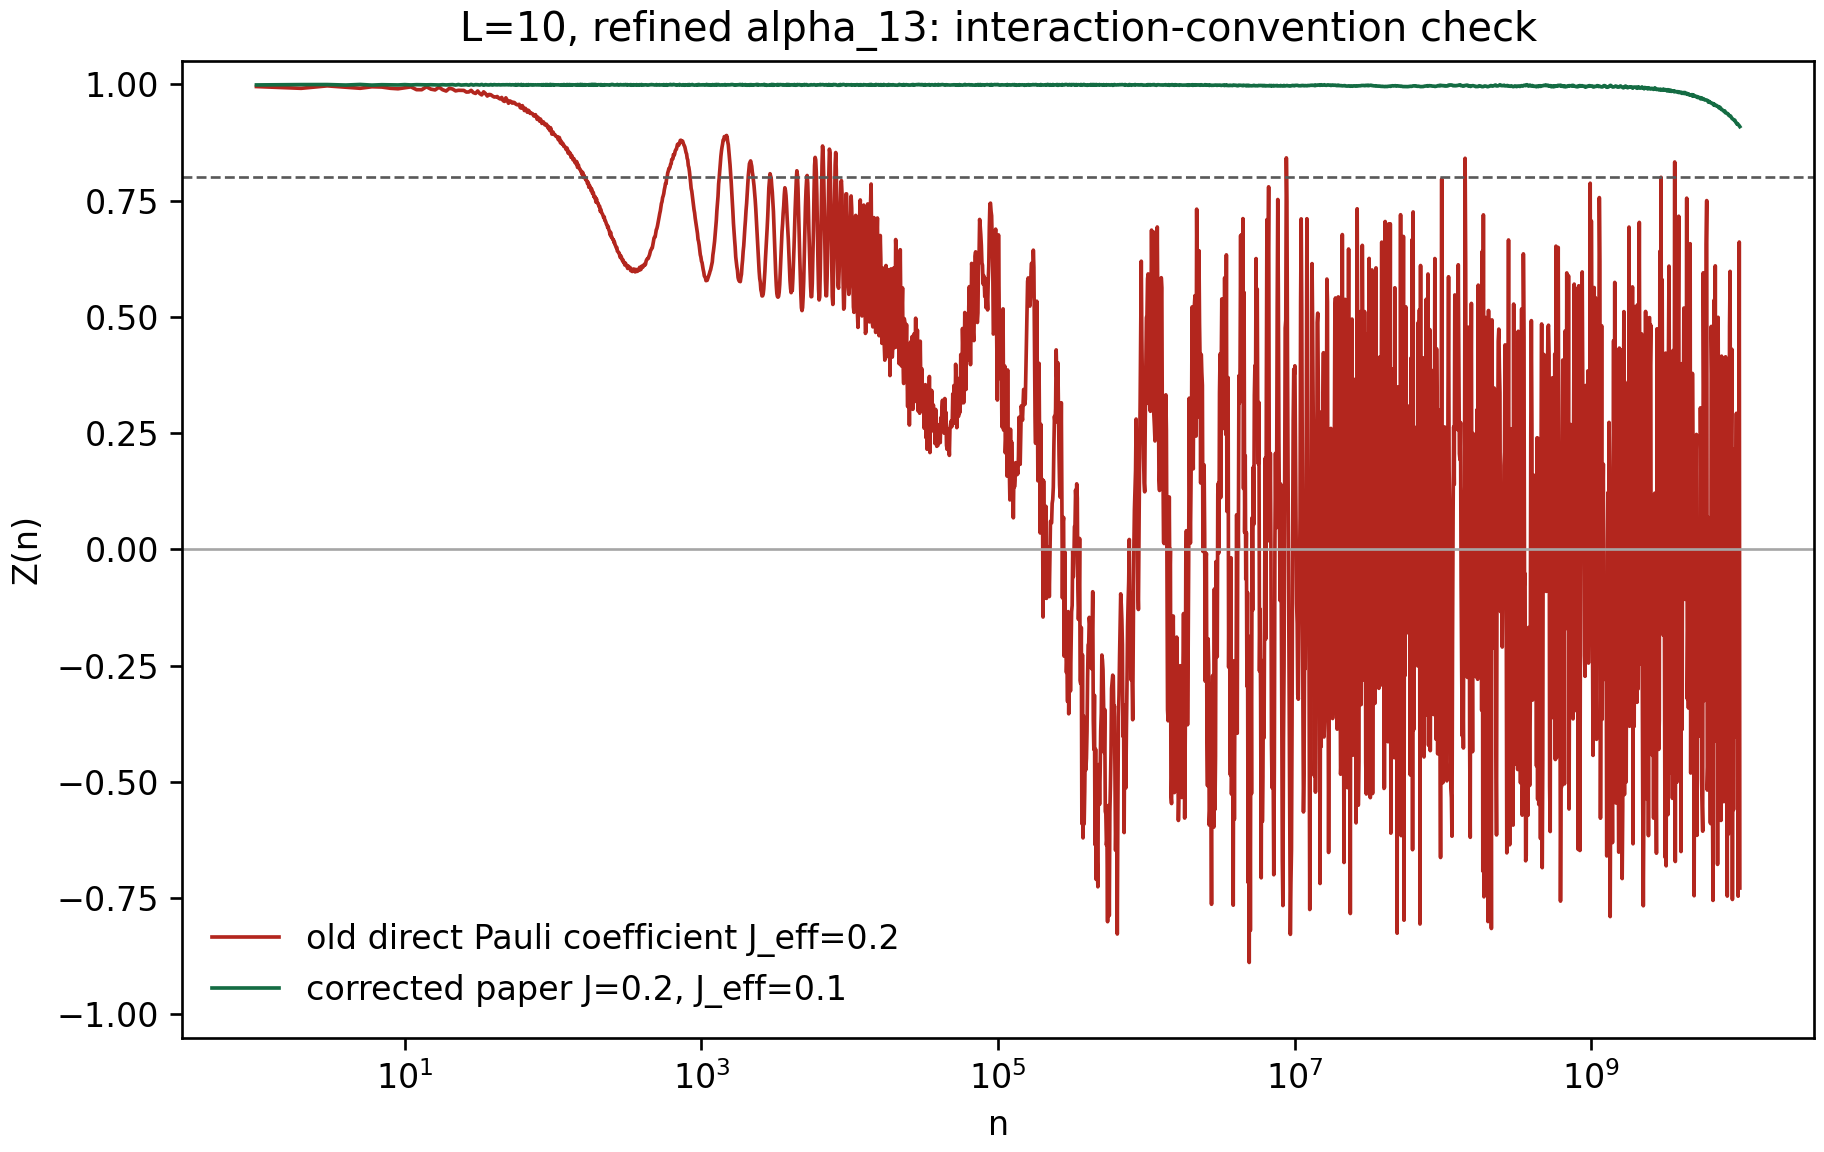
\includegraphics[width=0.92\linewidth]{interacting_l10_alpha13_j_convention_check.png}
\caption{Interaction-coefficient convention check for \(L=10\), refined \(\alpha_{13}\). The corrected convention maps the paper-label \(J=0.2\) to \(J_{\rm eff}=0.1\) for Pauli products.}
\label{fig:jconv}
\end{figure}

\subsection{Finite-size comparison}

The current-convention size comparison uses open boundaries, \(J_{\rm eff}=0.1\), fourth-order Magnus one-period Floquet construction, double precision, and logarithmic stroboscopic sampling. The refined \(\alpha_{13}\) case now shows the expected lifetime enhancement from \(L=8\) to \(L=10\), as shown in Fig.~\ref{fig:size-alpha13}. Using the operational threshold \(Z(n)<0.8\), \(L=8\) crosses at \(n=1.9967\times10^8\), while \(L=10\) crosses at \(n=1.5094\times10^{10}\).

\begin{figure}
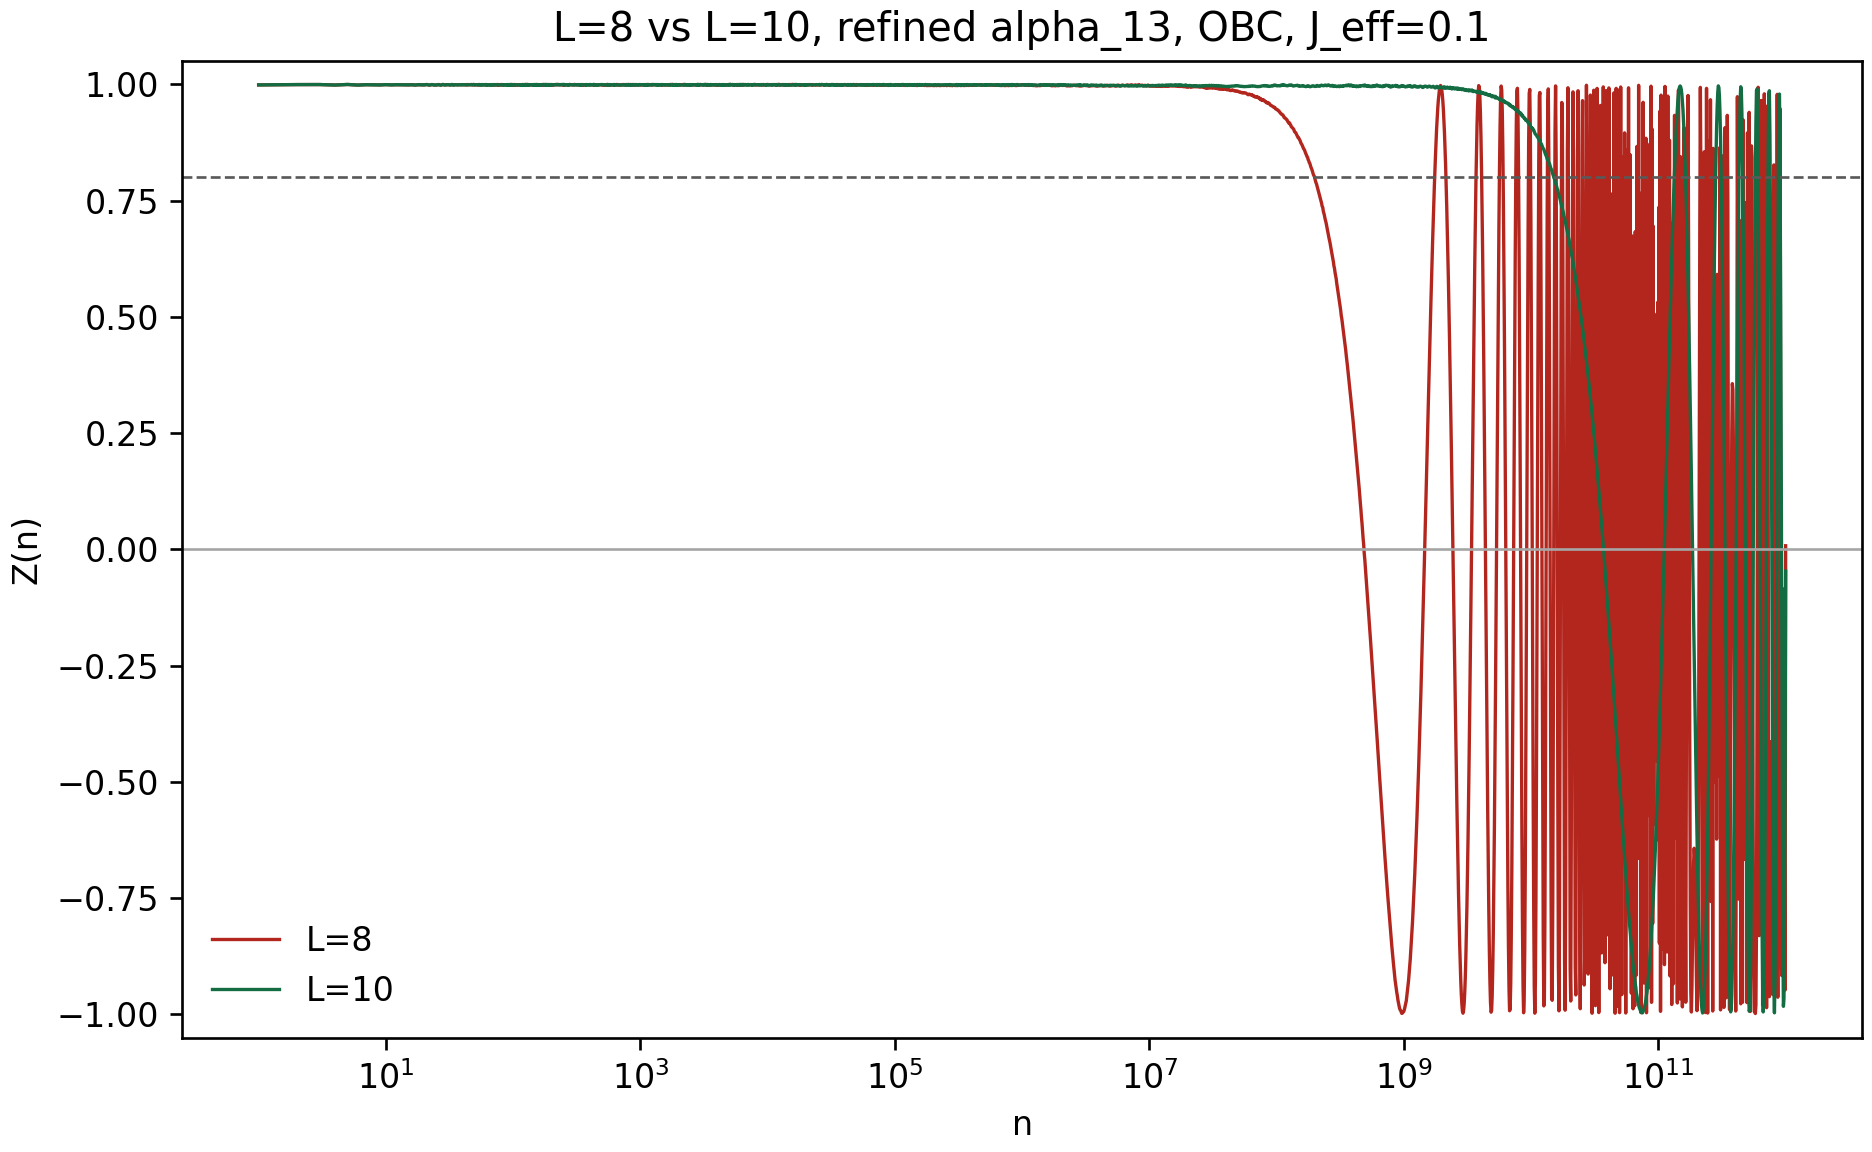
\includegraphics[width=0.92\linewidth]{interacting_l8_l10_alpha13_obc_comparison.png}
\caption{Open-boundary \(L=8\) and \(L=10\) comparison for refined \(\alpha_{13}\) using the corrected interaction convention. The larger chain has a much longer high-\(Z(n)\) interval.}
\label{fig:size-alpha13}
\end{figure}

The detuned \(\alpha=81.60\) result remains the main discrepancy. Figure~\ref{fig:size-alpha81} shows that both \(L=8\) and \(L=10\) drop quickly in the raw \(Z(n)\) trace. The threshold \(Z(n)<0.8\) is reached at \(n=3\) for both sizes, and the first negative sampled point occurs at \(n=65\) for \(L=8\) and \(n=78\) for \(L=10\). This is not consistent with a straightforward reading of the paper's Fig. 4(c).

\begin{figure}
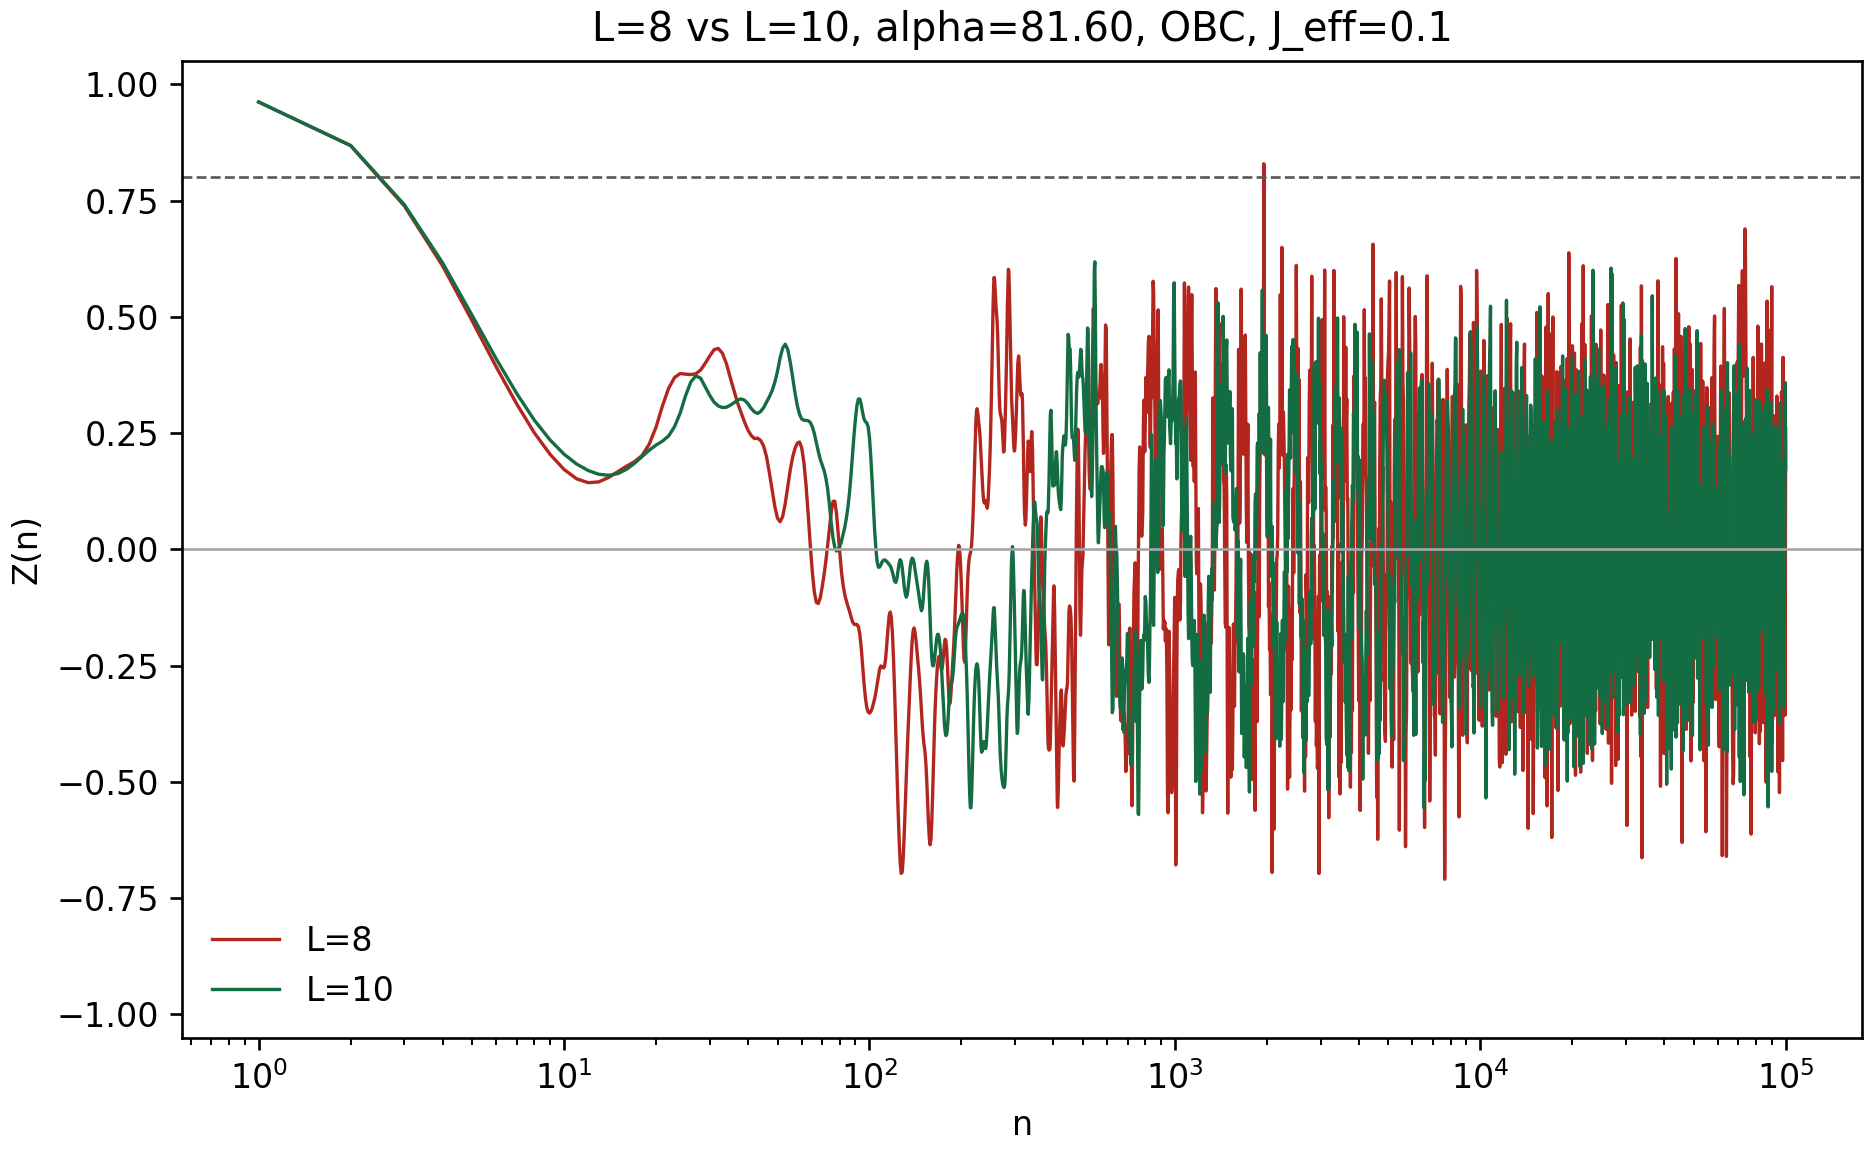
\includegraphics[width=0.92\linewidth]{interacting_l8_l10_alpha81p60_obc_comparison.png}
\caption{Open-boundary \(L=8\) and \(L=10\) comparison for detuned \(\alpha=81.60\). The raw \(Z(n)\) trace remains much less stable than expected from Fig. 4(c).}
\label{fig:size-alpha81}
\end{figure}

\begin{table}
\caption{Current-convention open-boundary stroboscopic thresholds.}
\label{tab:int-thresholds}
\begin{ruledtabular}
\begin{tabular}{lcccc}
case & \(L\) & \(n_{\max}\) & first \(Z<0.8\) & first \(Z<0\) \\
\hline
\(\alpha=81.60\) & 8 & \(10^5\) & 3 & 65 \\
\(\alpha=81.60\) & 10 & \(10^5\) & 3 & 78 \\
refined \(\alpha_{13}\) & 8 & \(10^{12}\) & \(1.9967\times10^8\) & \(4.8793\times10^8\) \\
refined \(\alpha_{13}\) & 10 & \(10^{12}\) & \(1.5094\times10^{10}\) & \(3.7263\times10^{10}\) \\
\end{tabular}
\end{ruledtabular}
\end{table}

\subsection{Boundary-condition checks}

The code originally used open boundaries. A periodic-boundary interface was added to test whether the detuned discrepancy was caused by boundary choice. For \(L=10\), refined \(\alpha_{13}\), periodic boundaries produced collapse and revival behavior, with first sampled \(Z(n)<0.8\) at \(n=7.8905\times10^8\) and first \(Z(n)<0\) at \(n=1.9224\times10^9\). For detuned \(\alpha=81.60\), both open and periodic boundaries still crossed \(Z(n)<0.8\) by \(n=3\). Boundary choice therefore does not explain the detuned Fig. 4(c) discrepancy.

\section{Reproducibility and HPC Workflow}

The local scripts are:
\begin{itemize}
\item \texttt{reproduction\_noninteracting/}\\
\texttt{reproduce\_noninteracting.py};
\item \texttt{reproduction\_interacting/}\\
\texttt{reproduce\_interacting.py}.
\end{itemize}
The core interacting cluster launcher is
\texttt{reproduction\_interacting/}\\
\texttt{run\_interacting\_hpc.sh}. It creates local \texttt{logs/} and \texttt{results/} directories before execution, records an environment snapshot, and excludes \texttt{gpuh01} because that node was known to have an older CUDA environment. The Slurm partition on the target cluster is \texttt{NV\_H100}, not \texttt{gpu}.

The main local validation commands are
\begin{verbatim}
python reproduction_noninteracting\reproduce_noninteracting.py
python reproduction_interacting\reproduce_interacting.py ^
  --params reproduction_interacting\params\interacting_params_hpc.json ^
  --output-root reproduction_interacting --device cuda
\end{verbatim}
and the report build command is
\begin{verbatim}
pdflatex -interaction=nonstopmode -halt-on-error comprehensive_report.tex
\end{verbatim}

\section{Assessment}

The reproduction is successful for the central symmetry-enforced mechanism and for the refined \(\alpha_{13}\) interacting stability after the interaction convention is corrected. The following points are now well supported:
\begin{enumerate}
\item The noninteracting two-level model displays clean two-period dynamics at the refined \(\alpha_{13}\).
\item The fractional-period projections show the expected intra-period eigenstate exchange.
\item The interacting short-time \(m_x(t)\) trace shows a half-drive-frequency peak.
\item The refined \(\alpha_{13}\) interacting chain has a longer \(Z(n)\) lifetime for \(L=10\) than for \(L=8\) under the corrected \(J_{\rm eff}=0.1\) convention.
\end{enumerate}

The main remaining risk is the detuned \(\alpha=81.60\) case. Under the current raw observable and both tested boundary conditions, the signal decays much faster than the paper's Fig. 4(c). This could reflect a difference in lifetime definition, observable processing, interaction normalization, or the exact numerical protocol used for the paper. Before making a publication-level claim about the detuned finite-size scaling, the next checks should test alternative interaction normalizations, sign-corrected local autocorrelations, envelope-based lifetime extraction, and \(L=12\) on the H100 if memory allows.

\section{Conclusion}

The project has now reproduced the main nonsymmorphic DTC mechanism and resolved the largest apparent contradiction in the refined-\(\alpha_{13}\) interacting data. The final corrected results support the expected DTC picture: accurate-period dynamics is much more stable than detuned dynamics, and the refined \(\alpha_{13}\) lifetime increases strongly from \(L=8\) to \(L=10\). The detuned Fig. 4(c) quantitative mismatch remains an explicit open problem rather than being hidden in the final report.

\begin{acknowledgments}
This report summarizes local RTX 4090 calculations, H100-oriented package preparation, and locally ingested H100 output generated during the reproduction workflow.
\end{acknowledgments}

\begin{thebibliography}{9}

\bibitem{hu2023dtc}
H. Hu, D. Fu, Y. Li, and S.-Q. Shen,
``Solvable model for discrete time crystal enforced by nonsymmorphic dynamical symmetry,''
Phys. Rev. Research \textbf{5}, L032024 (2023).

\bibitem{else2016floquet}
D. V. Else, B. Bauer, and C. Nayak,
``Floquet time crystals,''
Phys. Rev. Lett. \textbf{117}, 090402 (2016).

\bibitem{khemani2016phase}
V. Khemani, A. Lazarides, R. Moessner, and S. L. Sondhi,
``Phase structure of driven quantum systems,''
Phys. Rev. Lett. \textbf{116}, 250401 (2016).

\bibitem{abanin2017effective}
D. A. Abanin, W. De Roeck, W. W. Ho, and F. Huveneers,
``Effective Hamiltonians, prethermalization, and slow energy absorption in periodically driven many-body systems,''
Phys. Rev. B \textbf{95}, 014112 (2017).

\end{thebibliography}

\clearpage
\section*{Supplemental Material: Equations and Numerical Methods}

This supplemental section is a self-contained numerical guide. It is deliberately more explicit than the main report. The goal is that a reader who has seen undergraduate-level linear algebra, Taylor expansions, and ordinary differential equations can reconstruct the numerical methods used in the reproduction.

\subsection*{S1. Two-level Schrodinger equation as an ordinary differential equation}

For the noninteracting model the state is a two-component spinor
\begin{equation}
|\psi(t)\rangle =
\begin{pmatrix}
\psi_\uparrow(t)\\
\psi_\downarrow(t)
\end{pmatrix}.
\end{equation}
The Schrodinger equation is
\begin{equation}
i\hbar \frac{d}{dt}|\psi(t)\rangle=H_0(t)|\psi(t)\rangle.
\end{equation}
With \(\hbar=1\), this becomes the linear ordinary differential equation
\begin{equation}
\frac{d}{dt}|\psi(t)\rangle=A(t)|\psi(t)\rangle,\qquad
A(t)=-iH_0(t).
\label{eq:s1-ode}
\end{equation}
Using
\begin{equation}
\sigma_x=
\begin{pmatrix}
0&1\\
1&0
\end{pmatrix},\qquad
\sigma_y=
\begin{pmatrix}
0&-i\\
i&0
\end{pmatrix},
\end{equation}
Eq.~(\ref{eq:h0}) becomes
\begin{equation}
H_0(t)=
\begin{pmatrix}
0 & a(t)-ib(t)\\
a(t)+ib(t) & 0
\end{pmatrix},
\end{equation}
where
\begin{equation}
a(t)=\frac{1}{2}\Omega\sin t,\qquad
b(t)=\Omega\sin^2\left(\frac{t}{2}\right).
\end{equation}
The matrix \(H_0(t)\) is Hermitian, so \(A(t)=-iH_0(t)\) is anti-Hermitian:
\begin{equation}
A^\dagger(t)=-A(t).
\end{equation}
This one-line observation is important. The exact quantum propagator is unitary because it is generated by an anti-Hermitian matrix. A numerical method that preserves this anti-Hermitian exponential structure will preserve the norm much better than a generic polynomial time-stepper.

\subsection*{S2. Exact propagator and why time ordering matters}

If \(A(t)\) were constant over a time step, the exact solution would be
\begin{equation}
|\psi(t+\Delta t)\rangle=\exp[\Delta t A]|\psi(t)\rangle.
\end{equation}
For time-dependent \(A(t)\), the matrices at different times generally do not commute:
\begin{equation}
[A(t_1),A(t_2)]\neq0.
\end{equation}
The exact solution is therefore the time-ordered exponential
\begin{equation}
|\psi(t+\Delta t)\rangle
=\mathcal{T}\exp\left[\int_t^{t+\Delta t} A(s)\,ds\right]|\psi(t)\rangle.
\end{equation}
Here \(\mathcal{T}\) means that later-time matrices must be ordered to the left of earlier-time matrices. If all matrices commute, time ordering is unnecessary and the solution reduces to an ordinary exponential. The noncommuting case is why both Magnus methods and high-order Runge--Kutta methods are useful.

\subsection*{S3. Instantaneous eigenstates and stroboscopic projections}

At each time, \(H_0(t)\) has two instantaneous eigenstates. The paper writes them in a rotating basis, where the nonsymmorphic dynamical symmetry makes the eigenstates exchange after one period. Numerically we do not need to symbolically solve the full Heun-function problem. Instead we evolve the state and project it onto the basis used by the paper:
\begin{equation}
P_\chi(t)=|\langle \phi_\chi(t)|\psi(t)\rangle|^2,\qquad \chi=\pm.
\end{equation}
The exact-\(\alpha_n\) condition implies that an initial \(\phi_+(0)\) state has almost zero probability to return to \(\phi_+(0)\) after one period:
\begin{equation}
P_+(T)\simeq 0.
\end{equation}
In the reproduction this condition is used to refine the tabulated \(\alpha_{13}\). The resulting local value is
\begin{equation}
\alpha_{13}=80.04624211689759,
\end{equation}
with one-period return probability \(3.57\times10^{-18}\).

Integer-period projections show the period-doubled pattern, but they hide the motion inside each period. The reproduction therefore samples
\begin{equation}
t=nT,\quad nT+T/4,\quad nT+T/2,\quad nT+3T/4.
\end{equation}
This is why the final noninteracting data include both stroboscopic and fractional-period figures.

\subsection*{S4. Why RK4 uses four slopes}

Start from a general ordinary differential equation
\begin{equation}
\frac{dy}{dt}=f(t,y).
\label{eq:s4-ode}
\end{equation}
The exact one-step increment is not mysterious:
\begin{equation}
y(t+h)-y(t)=\int_t^{t+h} f(s,y(s))\,ds.
\label{eq:s4-integral}
\end{equation}
Thus every one-step ODE solver is, at some level, an approximation to this integral of the slope. Euler's method uses only the left-end slope. A midpoint method uses a slope near the center. Simpson-type quadrature suggests that a high-order method should combine beginning, midpoint, and endpoint slope information. RK4 does exactly this, but with a correction: the midpoint and endpoint states are unknown, so they must be predicted from previously computed slopes.

The classical RK4 choice is
\begin{align}
k_1&=f(t_n,y_n),\\
k_2&=f(t_n+h/2,y_n+hk_1/2),\\
k_3&=f(t_n+h/2,y_n+hk_2/2),\\
k_4&=f(t_n+h,y_n+hk_3),
\label{eq:s4-stages}
\end{align}
followed by
\begin{equation}
y_{n+1}=y_n+h(b_1k_1+b_2k_2+b_3k_3+b_4k_4).
\label{eq:s4-generic-rk}
\end{equation}
The two midpoint slopes have different roles. \(k_2\) uses an Euler prediction to the midpoint; \(k_3\) repeats the midpoint evaluation using the improved midpoint direction \(k_2\). Then \(k_4\) uses the improved midpoint direction to predict the endpoint. The four slopes therefore probe the beginning, two corrected midpoints, and the end of the interval.

\subsection*{S5. How the RK4 weights are determined}

The weights \(b_i\) are fixed by asking the method to reproduce the Taylor expansion of the exact flow. The exact solution has
\begin{equation}
y(t+h)=y(t)+hy'(t)+\frac{h^2}{2}y''(t)
+\frac{h^3}{6}y^{(3)}(t)
+\frac{h^4}{24}y^{(4)}(t)+O(h^5).
\label{eq:s5-taylor}
\end{equation}
A compact way to see where the classical RK4 weights come from is to apply the stages in Eq.~(\ref{eq:s4-stages}) to the scalar linear test equation
\begin{equation}
y'=\lambda y,\qquad z=h\lambda.
\end{equation}
For this equation,
\begin{align}
k_1&=\lambda y_n,\\
k_2&=\lambda\left(1+\frac{z}{2}\right)y_n,\\
k_3&=\lambda\left(1+\frac{z}{2}+\frac{z^2}{4}\right)y_n,\\
k_4&=\lambda\left(1+z+\frac{z^2}{2}+\frac{z^3}{4}\right)y_n.
\end{align}
Substituting into Eq.~(\ref{eq:s4-generic-rk}) gives an amplification polynomial
\begin{equation}
\frac{y_{n+1}}{y_n}
=1+z(b_1+b_2+b_3+b_4)
+z^2\left(\frac{b_2}{2}+\frac{b_3}{2}+b_4\right)
+z^3\left(\frac{b_3}{4}+\frac{b_4}{2}\right)
+z^4\left(\frac{b_4}{4}\right).
\end{equation}
The exact solution is \(e^z\), whose Taylor series is
\begin{equation}
e^z=1+z+\frac{z^2}{2}+\frac{z^3}{6}+\frac{z^4}{24}+O(z^5).
\end{equation}
Matching the coefficients through \(z^4\) gives
\begin{align}
b_1+b_2+b_3+b_4&=1,\\
\frac{b_2}{2}+\frac{b_3}{2}+b_4&=\frac{1}{2},\\
\frac{b_3}{4}+\frac{b_4}{2}&=\frac{1}{6},\\
\frac{b_4}{4}&=\frac{1}{24}.
\end{align}
Solving from bottom to top gives
\begin{equation}
b_4=\frac{1}{6},\qquad b_3=\frac{1}{3},\qquad
b_2=\frac{1}{3},\qquad b_1=\frac{1}{6}.
\end{equation}
This explains the familiar weighted average
\begin{equation}
y_{n+1}=y_n+\frac{h}{6}(k_1+2k_2+2k_3+k_4).
\label{eq:s5-rk4}
\end{equation}
In words, the two midpoint slopes carry twice the weight of the endpoint slopes because the midpoint information is what fixes the curvature terms in the Taylor series.

The scalar test equation is not the whole proof for a nonlinear time-dependent system, but it shows the basic logic. The full nonlinear derivation expands every stage \(k_i\) in powers of \(h\) and requires agreement with Eq.~(\ref{eq:s5-taylor}) for all elementary derivative structures. These requirements are the Runge--Kutta order conditions. For the classical choice
\begin{equation}
c_1=0,\quad c_2=c_3=\frac{1}{2},\quad c_4=1,\quad
a_{21}=a_{32}=\frac{1}{2},\quad a_{43}=1,
\end{equation}
the fourth-order conditions are satisfied by the weights above. They are summarized by the Butcher tableau
\begin{equation}
\begin{array}{c|cccc}
0&&&&\\
1/2&1/2&&&\\
1/2&0&1/2&&\\
1&0&0&1&\\
\hline
&1/6&1/3&1/3&1/6
\end{array}.
\end{equation}

\subsection*{S6. RK4 for matrix Schrodinger equations and why it is not unitary}

For the Schrodinger equation, \(y\) is the state vector \(\psi\), and
\begin{equation}
f(t,\psi)=-iH(t)\psi.
\end{equation}
Nothing in the RK4 construction requires \(y\) to be a scalar. If \(\psi\) has \(d\) components, then \(k_1,\ldots,k_4\) are also \(d\)-component vectors. Each stage is just a Hamiltonian matrix-vector product at a chosen time and predicted state.

Because Eq.~(\ref{eq:s5-rk4}) matches the exact Taylor expansion through \(h^4\), the local truncation error is
\begin{equation}
\epsilon_{\rm local}=O(h^5),
\end{equation}
and the global error over a fixed time interval is
\begin{equation}
\epsilon_{\rm global}=O(h^4).
\end{equation}
This is the numerical meaning of ``fourth order.''

However, RK4 is still a Taylor-polynomial method. For a constant Hamiltonian, \(A=-iH\), one RK4 step is
\begin{equation}
\psi_{n+1}=R(hA)\psi_n,
\end{equation}
with
\begin{equation}
R(z)=1+z+\frac{z^2}{2}+\frac{z^3}{6}+\frac{z^4}{24}.
\end{equation}
The exact propagator is \(e^{hA}\). If \(H\) is Hermitian, \(A\) is anti-Hermitian and \(e^{hA}\) is unitary. But the polynomial \(R(hA)\) is not exactly unitary. For one eigenmode \(z=ix\),
\begin{equation}
|R(ix)|^2=1-\frac{x^6}{72}+O(x^8).
\end{equation}
Thus RK4 can slowly lose or gain norm even when the exact quantum dynamics conserves norm exactly. This is why RK4 is useful as an independent high-order benchmark but not the preferred long-time unitary propagator. The reproduction monitors
\begin{equation}
\delta_{\rm norm}=\max_t
\left|\,\langle\psi(t)|\psi(t)\rangle-1\,\right|.
\end{equation}
Optional normalization after RK4 steps is a practical stabilizer for time traces; it does not turn RK4 into a structure-preserving unitary method.

\subsection*{S7. Why the Magnus expansion exists}

For the linear equation
\begin{equation}
\psi'(t)=A(t)\psi(t),
\end{equation}
the exact propagator is a time-ordered exponential. The Magnus method asks whether this time-ordered object can be written as a single ordinary exponential:
\begin{equation}
\psi(t+h)=\exp[\Omega(t,h)]\psi(t).
\label{eq:s7-single-exp}
\end{equation}
The answer is yes under standard smoothness and convergence conditions, and the price paid is that \(\Omega\) contains commutators.

One way to see the source of the commutators is to split the interval into small pieces. For two consecutive pieces with generators \(X\) and \(Y\),
\begin{equation}
e^X e^Y
=\exp\left(X+Y+\frac{1}{2}[X,Y]
+\frac{1}{12}[X,[X,Y]]
+\frac{1}{12}[Y,[Y,X]]+\cdots\right),
\label{eq:s7-bch}
\end{equation}
which is the Baker--Campbell--Hausdorff formula. If matrices commute, \(e^Xe^Y=e^{X+Y}\). If they do not commute, the commutators in Eq.~(\ref{eq:s7-bch}) are the correction terms required to compress a product of exponentials into one exponential. Taking the continuum limit of many small time slices gives the Magnus series:
\begin{align}
\Omega_1&=\int_t^{t+h} A(t_1)\,dt_1,\\
\Omega_2&=\frac{1}{2}\int_t^{t+h}dt_1
\int_t^{t_1}dt_2\,[A(t_1),A(t_2)],\\
\Omega_3&=\frac{1}{6}\int_t^{t+h}dt_1
\int_t^{t_1}dt_2
\int_t^{t_2}dt_3
\Big([A_1,[A_2,A_3]]+[A_3,[A_2,A_1]]\Big),
\end{align}
where \(A_j=A(t_j)\). This is the ``why'' behind the expansion: the usual integral \(\int A(t)dt\) is sufficient only when generators commute at different times.

\subsection*{S8. Why Magnus preserves unitarity}

For Schrodinger evolution \(A(t)=-iH(t)\) is anti-Hermitian. The sum and integral of anti-Hermitian matrices are anti-Hermitian. The commutator of two anti-Hermitian matrices is also anti-Hermitian:
\begin{equation}
\begin{aligned}
\relax
[A,B]^\dagger
&=(AB-BA)^\dagger\\
&=B^\dagger A^\dagger-A^\dagger B^\dagger\\
&=(-B)(-A)-(-A)(-B)\\
&=BA-AB\\
&=-[A,B].
\end{aligned}
\end{equation}
Therefore every retained term in a Magnus approximation is anti-Hermitian. If \(\Omega_{\rm num}^\dagger=-\Omega_{\rm num}\), then
\begin{equation}
U_{\rm num}=\exp(\Omega_{\rm num})
\end{equation}
is unitary:
\begin{equation}
U_{\rm num}^\dagger U_{\rm num}
=\exp(\Omega_{\rm num}^\dagger)\exp(\Omega_{\rm num})
=\exp(-\Omega_{\rm num})\exp(\Omega_{\rm num})=I.
\end{equation}
This is the key structural difference from RK4. RK4 approximates \(e^{hA}\) by a polynomial. Magnus approximates the generator \(\Omega\) and then exponentiates it, preserving the correct geometric form of quantum time evolution.

\subsection*{S9. Why the fourth-order Gauss--Legendre Magnus formula has this form}

The reproduction uses a fourth-order two-point Gauss--Legendre Magnus step. Let the midpoint of the step be \(t_m=t+h/2\), and define
\begin{equation}
t_1=t_m-\frac{\sqrt{3}}{6}h,\qquad
t_2=t_m+\frac{\sqrt{3}}{6}h,
\end{equation}
with
\begin{equation}
A_1=A(t_1),\qquad A_2=A(t_2).
\end{equation}
The first Magnus term is the integral of \(A(t)\). Two-point Gauss--Legendre quadrature is chosen because it integrates polynomials through cubic order exactly:
\begin{equation}
\Omega_1=\int_t^{t+h}A(s)\,ds
=\frac{h}{2}(A_1+A_2)+O(h^5).
\label{eq:s9-omega1}
\end{equation}
The node distance \(\sqrt{3}/6\) is fixed by this fourth-order quadrature requirement. In midpoint coordinates \(\tau=s-t_m\),
\begin{equation}
A(t_m+\tau)=A_0+\tau \dot A_0+\frac{\tau^2}{2}\ddot A_0+\frac{\tau^3}{6}A_0^{(3)}+\cdots.
\end{equation}
Using symmetric nodes \(\tau=\pm(\sqrt{3}/6)h\) cancels all odd terms and reproduces the \(h^3\ddot A_0/24\) contribution to the exact integral. This explains the Gauss nodes.

The commutator coefficient is fixed by the second Magnus term. Keeping only the leading noncommuting contribution,
\begin{equation}
[A(t_m+\tau_1),A(t_m+\tau_2)]
=(\tau_2-\tau_1)[A_0,\dot A_0]+O(h^2).
\end{equation}
Substituting this into \(\Omega_2\) gives
\begin{equation}
\Omega_2=-\frac{h^3}{12}[A_0,\dot A_0]+O(h^5).
\label{eq:s9-omega2-leading}
\end{equation}
Now expand the commutator of the two Gauss-node matrices:
\begin{equation}
[A_1,A_2]
=\frac{\sqrt{3}}{3}h[A_0,\dot A_0]+O(h^3).
\end{equation}
Therefore
\begin{equation}
-\frac{\sqrt{3}h^2}{12}[A_1,A_2]
=-\frac{h^3}{12}[A_0,\dot A_0]+O(h^5),
\end{equation}
which matches Eq.~(\ref{eq:s9-omega2-leading}). This is why the fourth-order Gauss--Legendre Magnus generator is
\begin{equation}
\Omega_{\rm GL4}
=\frac{h}{2}(A_1+A_2)
-\frac{\sqrt{3}h^2}{12}[A_1,A_2].
\label{eq:s9-magnus}
\end{equation}
The formula is not an empirical correction. The first term is fixed by fourth-order quadrature of the ordinary integral, and the second term is fixed by the leading noncommutative part of the exact Magnus expansion.

The numerical update is
\begin{equation}
\psi_{n+1}=\exp(\Omega_{\rm GL4})\psi_n.
\end{equation}
For smooth \(A(t)\), the local error is \(O(h^5)\) and the global error is \(O(h^4)\). Thus Magnus4 and RK4 have the same formal order, but Magnus4 preserves unitarity step by step when \(H(t)\) is Hermitian.

\subsection*{S10. Comparing RK4 and Magnus in this reproduction}

The reason to use both methods is now clear. RK4 is a high-order polynomial slope method whose coefficients are fixed by Taylor matching. It is easy to implement and works for general vector ODEs, so it is a useful independent check. Magnus4 is a high-order exponential method whose coefficients are fixed by time ordering and noncommutativity. It is more expensive, but it respects the unitary structure of Schrodinger evolution.

In the two-level calculation, \(\Omega_{\rm GL4}\) is only \(2\times2\), so the matrix exponential is cheap. In the interacting Floquet construction, \(\Omega_{\rm GL4}\) is a \(2^L\times2^L\) matrix for the dense one-period calculation. The step matrices are multiplied to build
\begin{equation}
U(T)\approx U_{N-1}\cdots U_1U_0,\qquad
U_j=\exp(\Omega_{{\rm GL4},j}).
\end{equation}
Since each \(U_j\) is unitary up to floating-point matrix-exponential error, the product is also unitary up to roundoff. This is why the long-time stroboscopic Floquet calculation uses Magnus4 rather than RK4.

\subsection*{S11. Many-body basis and Hamiltonian action}

For the interacting chain the computational basis is the \(z\)-basis
\begin{equation}
|b_{L-1}\cdots b_1b_0\rangle,\qquad b_i\in\{0,1\}.
\end{equation}
The Hilbert-space dimension is \(2^L\). A basis index is stored as an integer
\begin{equation}
q=\sum_{i=0}^{L-1}b_i2^i.
\end{equation}
Acting with \(\sigma_x^i\) flips bit \(i\):
\begin{equation}
q\mapsto q\oplus 2^i,
\end{equation}
where \(\oplus\) is bitwise exclusive-or. Acting with \(\sigma_y^i\) also flips the bit but adds a phase:
\begin{equation}
\sigma_y|0\rangle=i|1\rangle,\qquad
\sigma_y|1\rangle=-i|0\rangle.
\end{equation}
This lets the code apply the Hamiltonian to the state vector without building a dense many-body Hamiltonian for ordinary time traces.

The interaction term is diagonal in the \(x\)-flipped representation:
\begin{equation}
\sigma_x^i\sigma_x^{i+1}|q\rangle
=|q\oplus2^i\oplus2^{i+1}\rangle.
\end{equation}
For open boundaries the bond list is
\begin{equation}
(1,2),(2,3),\ldots,(L-1,L).
\end{equation}
For periodic boundaries the additional bond \((L,1)\) is included.

\subsection*{S12. Initial state and observable evaluation}

The all-\(+x\) product state is represented in the \(z\)-basis as
\begin{equation}
|+x\rangle^{\otimes L}
=2^{-L/2}\sum_q |q\rangle.
\end{equation}
If a site is initialized in \(|-x\rangle\), the code changes the sign of amplitudes with \(b_i=1\). The current production runs use the all-\(+x\) case because it directly maximizes \(m_x(0)\) and matches the main-text Fig. 4 convention.

For a normalized state vector \(\psi_q\), the local \(x\)-magnetization is
\begin{equation}
\langle\sigma_x^i\rangle
=\sum_q \psi_q^*\psi_{q\oplus2^i}.
\end{equation}
The averaged magnetization and DTC diagnostic are
\begin{equation}
m_x(nT)=\frac{1}{L}\sum_i\langle\sigma_x^i(nT)\rangle,
\qquad
Z(n)=(-1)^n m_x(nT).
\end{equation}

\subsection*{S13. Long-time Floquet sampling}

Directly evolving every period up to \(n=10^{10}\) or \(10^{12}\) is impractical. The reproduction instead constructs the one-period Floquet matrix \(U(T)\) and uses logarithmic sample points. For each sample \(n\), the state is computed by matrix-power action:
\begin{equation}
|\psi(nT)\rangle=U(T)^n|\psi(0)\rangle.
\end{equation}
The sample set contains a dense linear prefix for early-time behavior and logarithmically spaced points for long-time decay. This keeps the CSV files small while preserving the lifetime-scale information.

For \(L=10\), \(U(T)\) is a \(1024\times1024\) complex matrix, which is feasible on a local RTX 4090 and on the H100 node. For \(L=12\), the dimension becomes \(4096\), so memory and runtime must be checked before launching long sweeps.

\subsection*{S14. Practical reproduction checklist}

A minimal local reproduction proceeds as follows:
\begin{enumerate}
\item Set \(\hbar=1\), \(\omega=1\), \(T=2\pi\), and \(\Omega=\alpha/8\).
\item For the noninteracting model, evolve Eq.~(\ref{eq:s1-ode}) using both Eq.~(\ref{eq:s9-magnus}) and RK4.
\item Refine \(\alpha_{13}\) by minimizing the one-period return probability.
\item For the interacting model, initialize \(|+x\rangle^{\otimes L}\).
\item Use the paper-label \(J=0.2\) but apply the Pauli-product coefficient \(J_{\rm eff}=0.1\).
\item Build \(U(T)\) with fourth-order Magnus steps and sample \(Z(n)\) at linear-plus-logarithmic periods.
\item Compare \(Z(n)\) thresholds across \(L\), boundary conditions, and \(\alpha\).
\end{enumerate}
The final data show that refined \(\alpha_{13}\) passes this checklist and has the expected longer lifetime at larger \(L\). The detuned \(\alpha=81.60\) case remains the only substantial quantitative mismatch with the paper's plotted Fig. 4(c).

\end{document}
